
\chapter{Quantification of PCA/PLS-DA Class Separations}

\begin{quote}
{\it
  People want to see patterns in the world. ... So important is this skill
  that we apply it everywhere, warranted or not.}
\\\\
 -- Benoit Mandelbrot
\end{quote}

\section{Introduction}

\begin{doublespace}
The importance placed on interpretation of PCA, PLS-DA and OPLS-DA scores plots
necessitates the use of quantitative procedures to determine the significance
of separations between multiple experimental groups in scores space. However,
no de facto protocol or metric exists to provide a means of reporting the
degree or significance of group separation
\cite{werth:abio2010,goodpaster:abio2010,goodpaster:cils2011}.
Anderson et al. used the $J_2$ criterion
\cite{anderson:metab2008,koutroumbas2006} to assess the quality of
resulting scores clusters according to the average withing-group and
between-group scatters for all groups. However, the $J_2$ metric only provides
an overall estimate of group separation without fine-grained information on
each pair of groups \cite{koutroumbas2006}. A similar problem exists
with the related Davies-Bouldin index \cite{davies:ieee1979}, which
chooses a worst-case estimate of group overlap as its figure of merit. Dixon
et al. \cite{dixon:jchemo2009} also comprehensively reported the
performances of four cluster separation indices based on modifications of
metrics used to validate separation for unsupervised clustering algorithms.
Alternatively, the PCAtoTree protocol constructs dendrograms from Euclidean
distance matrices computed from PCA scores for the PHYLIP
\cite{felsenstein:clad1989} software suite using a bootstrapping routine to
determine branch node significance \cite{werth:abio2010,retief:mmbio2000}.
However, it was recently shown that hypothesis testing using a Mahalanobis
distance metric and the $T^2$ and $F$ distributions can provide a statistical
means of quantifying group similarity \cite{goodpaster:cils2011}, suggesting
the possibility of returning $p$ values for full statistical quantitation of
group separations in scores space.
\end{doublespace}

\section{Materials and Methods}

\begin{doublespace}
The methods described below were implemented in software using the C
programming language with minimal external dependencies, so the programs
may be compiled and executed on any modern GNU/Linux distribution.
\end{doublespace}

\subsection{Probability Calculation}

\begin{doublespace}
Under the assumption that each group in the scores space is distributed as a
multivariate normal random variable, the separations between groups may be
calculated using the squared Mahalanobis distance metric
\cite{mahalanobis:pnisi1936}:

\begin{equation}
D_M^2 =
  (\mathbf{u}_j - \mathbf{u}_i)^T
  \mathbf{S}_p^{-1}
  (\mathbf{u}_j - \mathbf{u}_i)
\end{equation}

In the above equation, $\mathbf{u}_i, \mathbf{u}_j \in \mathbb{R}^p$ are the
$p$-variate sample means of groups $i$ and $j$, respectively, and
$\mathbf{S}_p \in \mathbb{R}^{p \times p}$ is the pooled variance-covariance
matrix, a weighted sum of the covariance matrices from groups $i$ and
$j$:

\begin{equation}
\mathbf{S}_p = \frac{n_i \mathbf{S}_i + n_j \mathbf{S}_j}{n_i + n_j}
\end{equation}

where $n_i$ and $n_j$ are the number of observations in groups $i$ and $j$,
respectively. The Mahalanobis distance may then be related to a Hotelling's
$T^2$ statistic by the following scaling \cite{mardia1979}:

\begin{equation}
T^2 = \left( \frac{n_i n_j}{n_i + n_j} \right) D_M^2
\end{equation}

This $T^2$ statistic is an extension of the Student's $t$ statistic to
hypothesis tests in multiple dimensions, and may be related to an $F$
distribution by a final scaling \cite{mardia1979}:

\begin{equation}
x_F =
  \frac{n_i + n_j - p - 1}{p (n_i + n_j - 2)} T^2 \sim
  F(p, n_i + n_j - p - 1)
\end{equation}

It can be seen from this final relation that evaluation of the complement of
the cumulative $F$-distribution function at $x_F$ yields the $p$ value for
accepting the null hypothesis: the points in groups $i$ and $j$ are in fact
drawn from the same distribution.
\end{doublespace}

\begin{figure}[ht!]
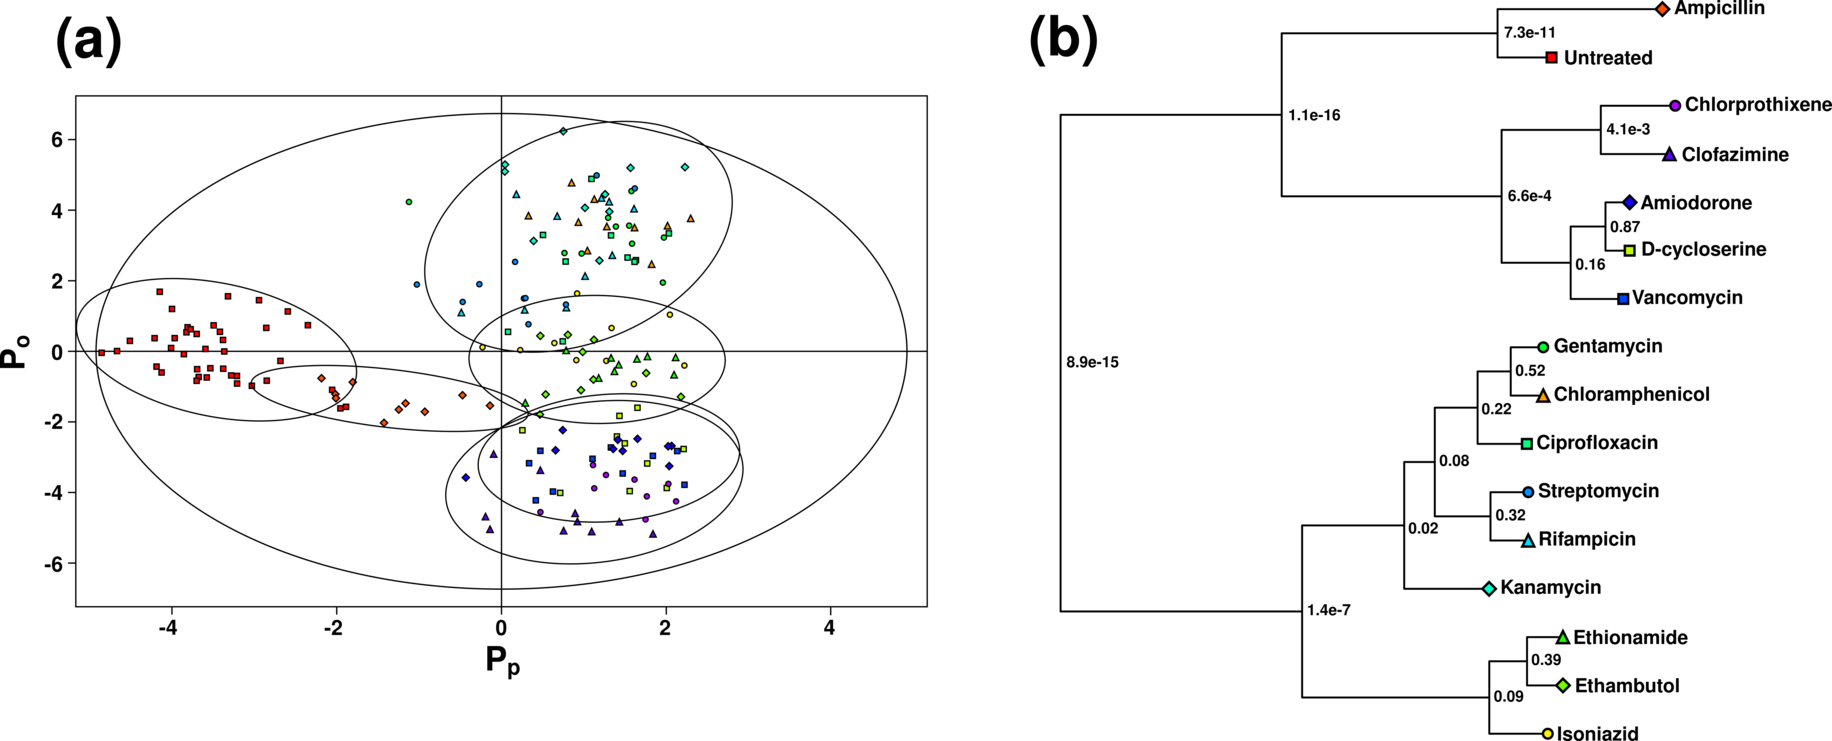
\includegraphics[width=6.5in]{figs/utils/01.png}
\caption
      [Confidence Ellipses and $p$-dendrogram of Example OPLS-DA Scores.]{
  {\bf Confidence Ellipses and $p$-dendrogram of Example OPLS-DA Scores.}
  \\
  ({\bf A}) 2D OPLS-DA scores plot illustrating 95\% confidence ellipses for
  a model having one predictive (PLS) and one orthogonal (OSC) component. The
  symbol shape and color each point correpond to the groups in ({\bf B}).
  Discrimination in the first component is between wild-type and
  antibiotic-treated {\it Mycobacterium smegmatis}, and separations along the
  second component indicate metabolic differences between different antibiotic
  treatments. The antibiotics cluster together based on a shared biological
  target (cell wall synthesis, mycolic acid biosynthesis, or transcription,
  translation and DNA supercoiling). ({\bf B}) Dendrogram generated from the
  scores in ({\bf A}) using Mahalanobis distances, with $p$ values for the null
  hypothesis reported at each branch.
}
\end{figure}

\subsection{Dendrogram Generation}

\begin{doublespace}
The implementation of the tree-generation procedure is a classical UPGMA
algorithm \cite{sokal:uksci1958}. When $p$ values are reported at
each branch point, a single tree is generated based on the matrix of
Mahalanobis distances between groups. In the case of bootstrapped trees, the
groups are randomly resampled with replacement while preserving group size.
The desired number of trees is then generated using Euclidean distances
between group means. The final tree used to report bootstrap probabilities
is built using a Euclidean distance matrix calculated from the original
(non-resampled) dataset.
\end{doublespace}

\subsection{Confidence Ellipse Calculation}

\begin{doublespace}
When viewing PCA and PLS-DA scores plots, it was common practice to apply
hand-drawn ellipses to inform group membership, or even to omit such ellipses
entirely. This may lead to inconsistent or erroneous interpretation of
experimental results. Instead, the fact that the Mahalanobis distances of a
set of $p$-variate points from their sample mean follow a $\chi^2$ distribution
having $p$ degrees of freedom \cite{hotelling:ams1931} may be leveraged
to estimate 95\% confidence ellipses for scores in any number of dimensions.
The sample mean $\mathbf{u}$ and sample covariance matrix $\mathbf{S}$ for each
group must first be calculated from its scores-space data. Then, each group
covariance matrix is decomposed into its eigenvalues and eigenvectors,

\begin{equation}
\mathbf{S} = \mathbf{Q} \mathbf{\Lambda} \mathbf{Q}^{-1}
\end{equation}

where $\mathbf{Q} \in \mathbb{R}^{p \times p}$ is an orthogonal matrix holding
the eigenvectors of $\mathbf{S}$, and
$\mathbf{\Lambda} \in \mathbb{R}^{p \times p}$ is a diagonal matrix holding the
corresponding eigenvalues of $\mathbf{S}$.

For the case of two-dimensional scores data, the 95\% confidence ellipse for a
group is as follows:
\end{doublespace}

\begin{equation}
\begin{bmatrix}
x(t) \\
y(t)
\end{bmatrix}
 = \mathbf{u} + \mathbf{Q} \sqrt{\mathbf{\Lambda} F_{0.95,2}^{-1}}
\begin{bmatrix}
\cos(t) \\
\sin(t)
\end{bmatrix}
\end{equation}

\begin{doublespace}
where $F_{0.95,2}^{-1}$ is the value of the inverse $\chi^2$ cumulative
distribution function at $\alpha = 0.05$ and two degrees of freedom, and the
square-root is taken element-wise over $\mathbf{\Lambda}$. Similarly, a
three-dimensional (3D) confidence ellipsoid may be obtained from the
following parametric equation:
\end{doublespace}

\begin{equation}
\begin{bmatrix}
x(u,v) \\
y(u,v) \\
z(u,v)
\end{bmatrix}
 = \mathbf{u} + \mathbf{Q} \sqrt{\mathbf{\Lambda} F_{0.95,3}^{-1}}
\begin{bmatrix}
\cos(u) \cos(v) \\
\cos(u) \sin(v) \\
\sin(v)
\end{bmatrix}
\end{equation}

\begin{doublespace}
where the parameters $t$, $u$ and $v$ are all evaluated on $(0,2\pi)$. These
methods allow for the inclusion of confidence regions onto two- and
three-dimensional scores plots that reflect the 95\% membership boundaries
for each group. The approach assumes normally distributed within-group errors.
Figures 8.1A and 8.2 illustrate the inclusion of these group confidence regions
in representative PCA and OPLS-DA scores, respectively. The ellipses and
ellipsoids clearly define statistically significant class separation and also
provide an example in which multiple groups actually belong to the same
underlying biological classification.
\end{doublespace}

\begin{SCfigure}
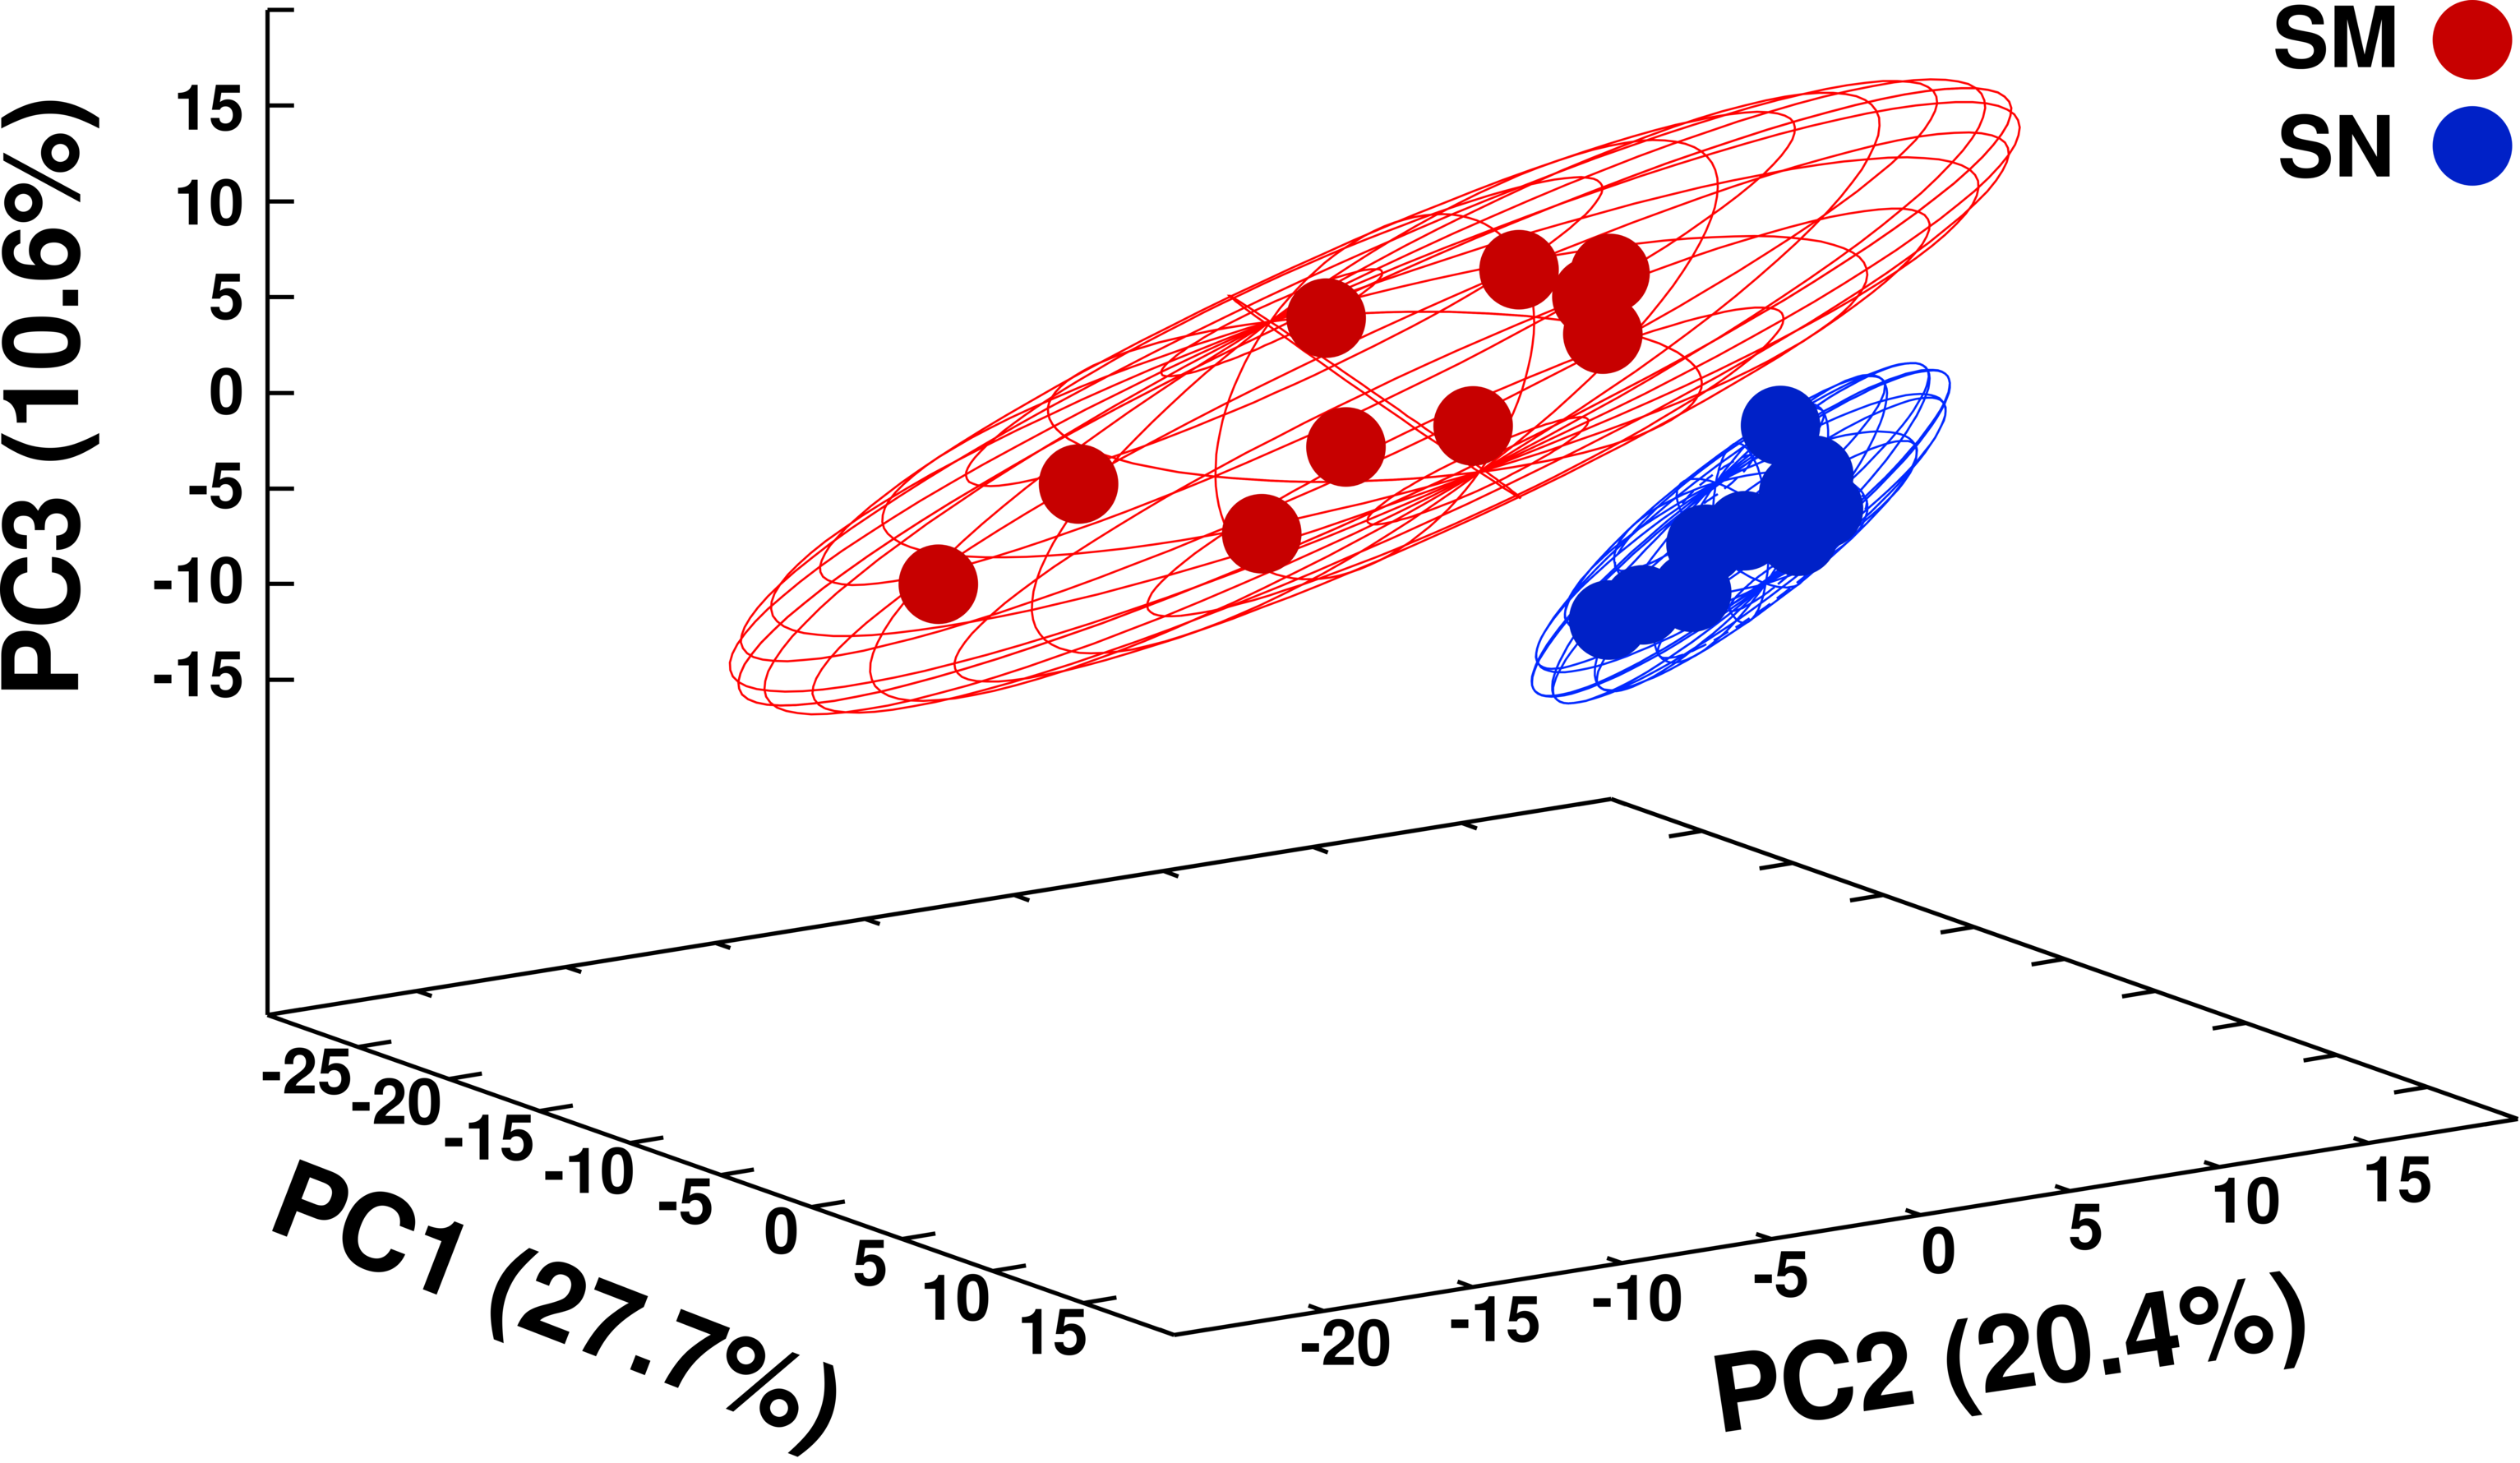
\includegraphics[width=3.5in]{figs/utils/02.png}
\caption
      [Confidence Ellipsoids from PCA Scores.]{
  {\bf Confidence Ellipsoids from PCA Scores.}
  \\
  3D PCA scores plot with superimposed 95\% confidence ellipsoids drawn as
  meshes containing group points. The ellipsoids define the statistical
  significance of class separation and provide an illustration where two
  groups are distinct in three-dimensional scores space.
}
\end{SCfigure}

\section{Results and Discussion}

\begin{doublespace}
The described PCA utilities software package consists of a set of standalone
C programs that generate dendrograms from PCA, PLS-DA and OPLS-DA scores,
report $p$ values and boostrap numbers on tree branches, and incorporate
confidence ellipses/ellipsoids into scores plots. The $p$ values reported for
every pair of distinct groups in scores space provide a truly quantitative
means to discuss group separations. Support for the generation of dendrograms
with these $p$ values at each branch point is also included as an alternative
answer to the bootstrap for answering the question of tree uniqueness. This
eliminates the prior dependence on PHYLIP \cite{retief:mmbio2000}
reported for the original PCAtoTree \cite{werth:abio2010} software
package. The reporting of $p$ values is complementary to bootstrapping methods
in cases of highly overlapped groups, in that it provides a more direct,
interpretable quantitation of group separation.
\\\\
In comparison with PCAtoTree, the PCA utilities software package now uses
Mahalanobis distances because this metric is more appropriate for multivariate
data. De Maesschalck et al. \cite{demaesschalck:cils2000} provide an
exceptional introduction to the use of Mahalanobis distances with PCA.
Specifically, Mahalanobis distances account for different variances in each
scores-space direction ($t_1$, $t_2$, $t_3$, \emph{etc.}) and are invariant
to scaling transformations. This accounting for variances-covariance structure
ensures that the use of a Mahalanobis distance metric for dendrogram generation
includes cluster shape and orientation in the analysis of group separation.
Also, Mahalanobis distances calculated between groups in PCA scores space will
closely approximate those calculated from the original data matrix while
avoiding possible multicollinearities among the original variables. This is
not true of Mahalanobis distances in PLS or OPLS scores space, because of the
underlying supervision of the PLS algorithm. These features differ from the
Euclidean distance metric, which is a special case of the Mahalanobis metric
that arises when the group covariance matrices equal the identity matrix.
Figure 8.1B illustrates the dendrogram structure based on the use of
Mahalanobis distances determined from a set of scores, and Figure 8.3 shows the
dendrogram structure based on Euclidean distances from the same scores.
\end{doublespace}

\begin{SCfigure}
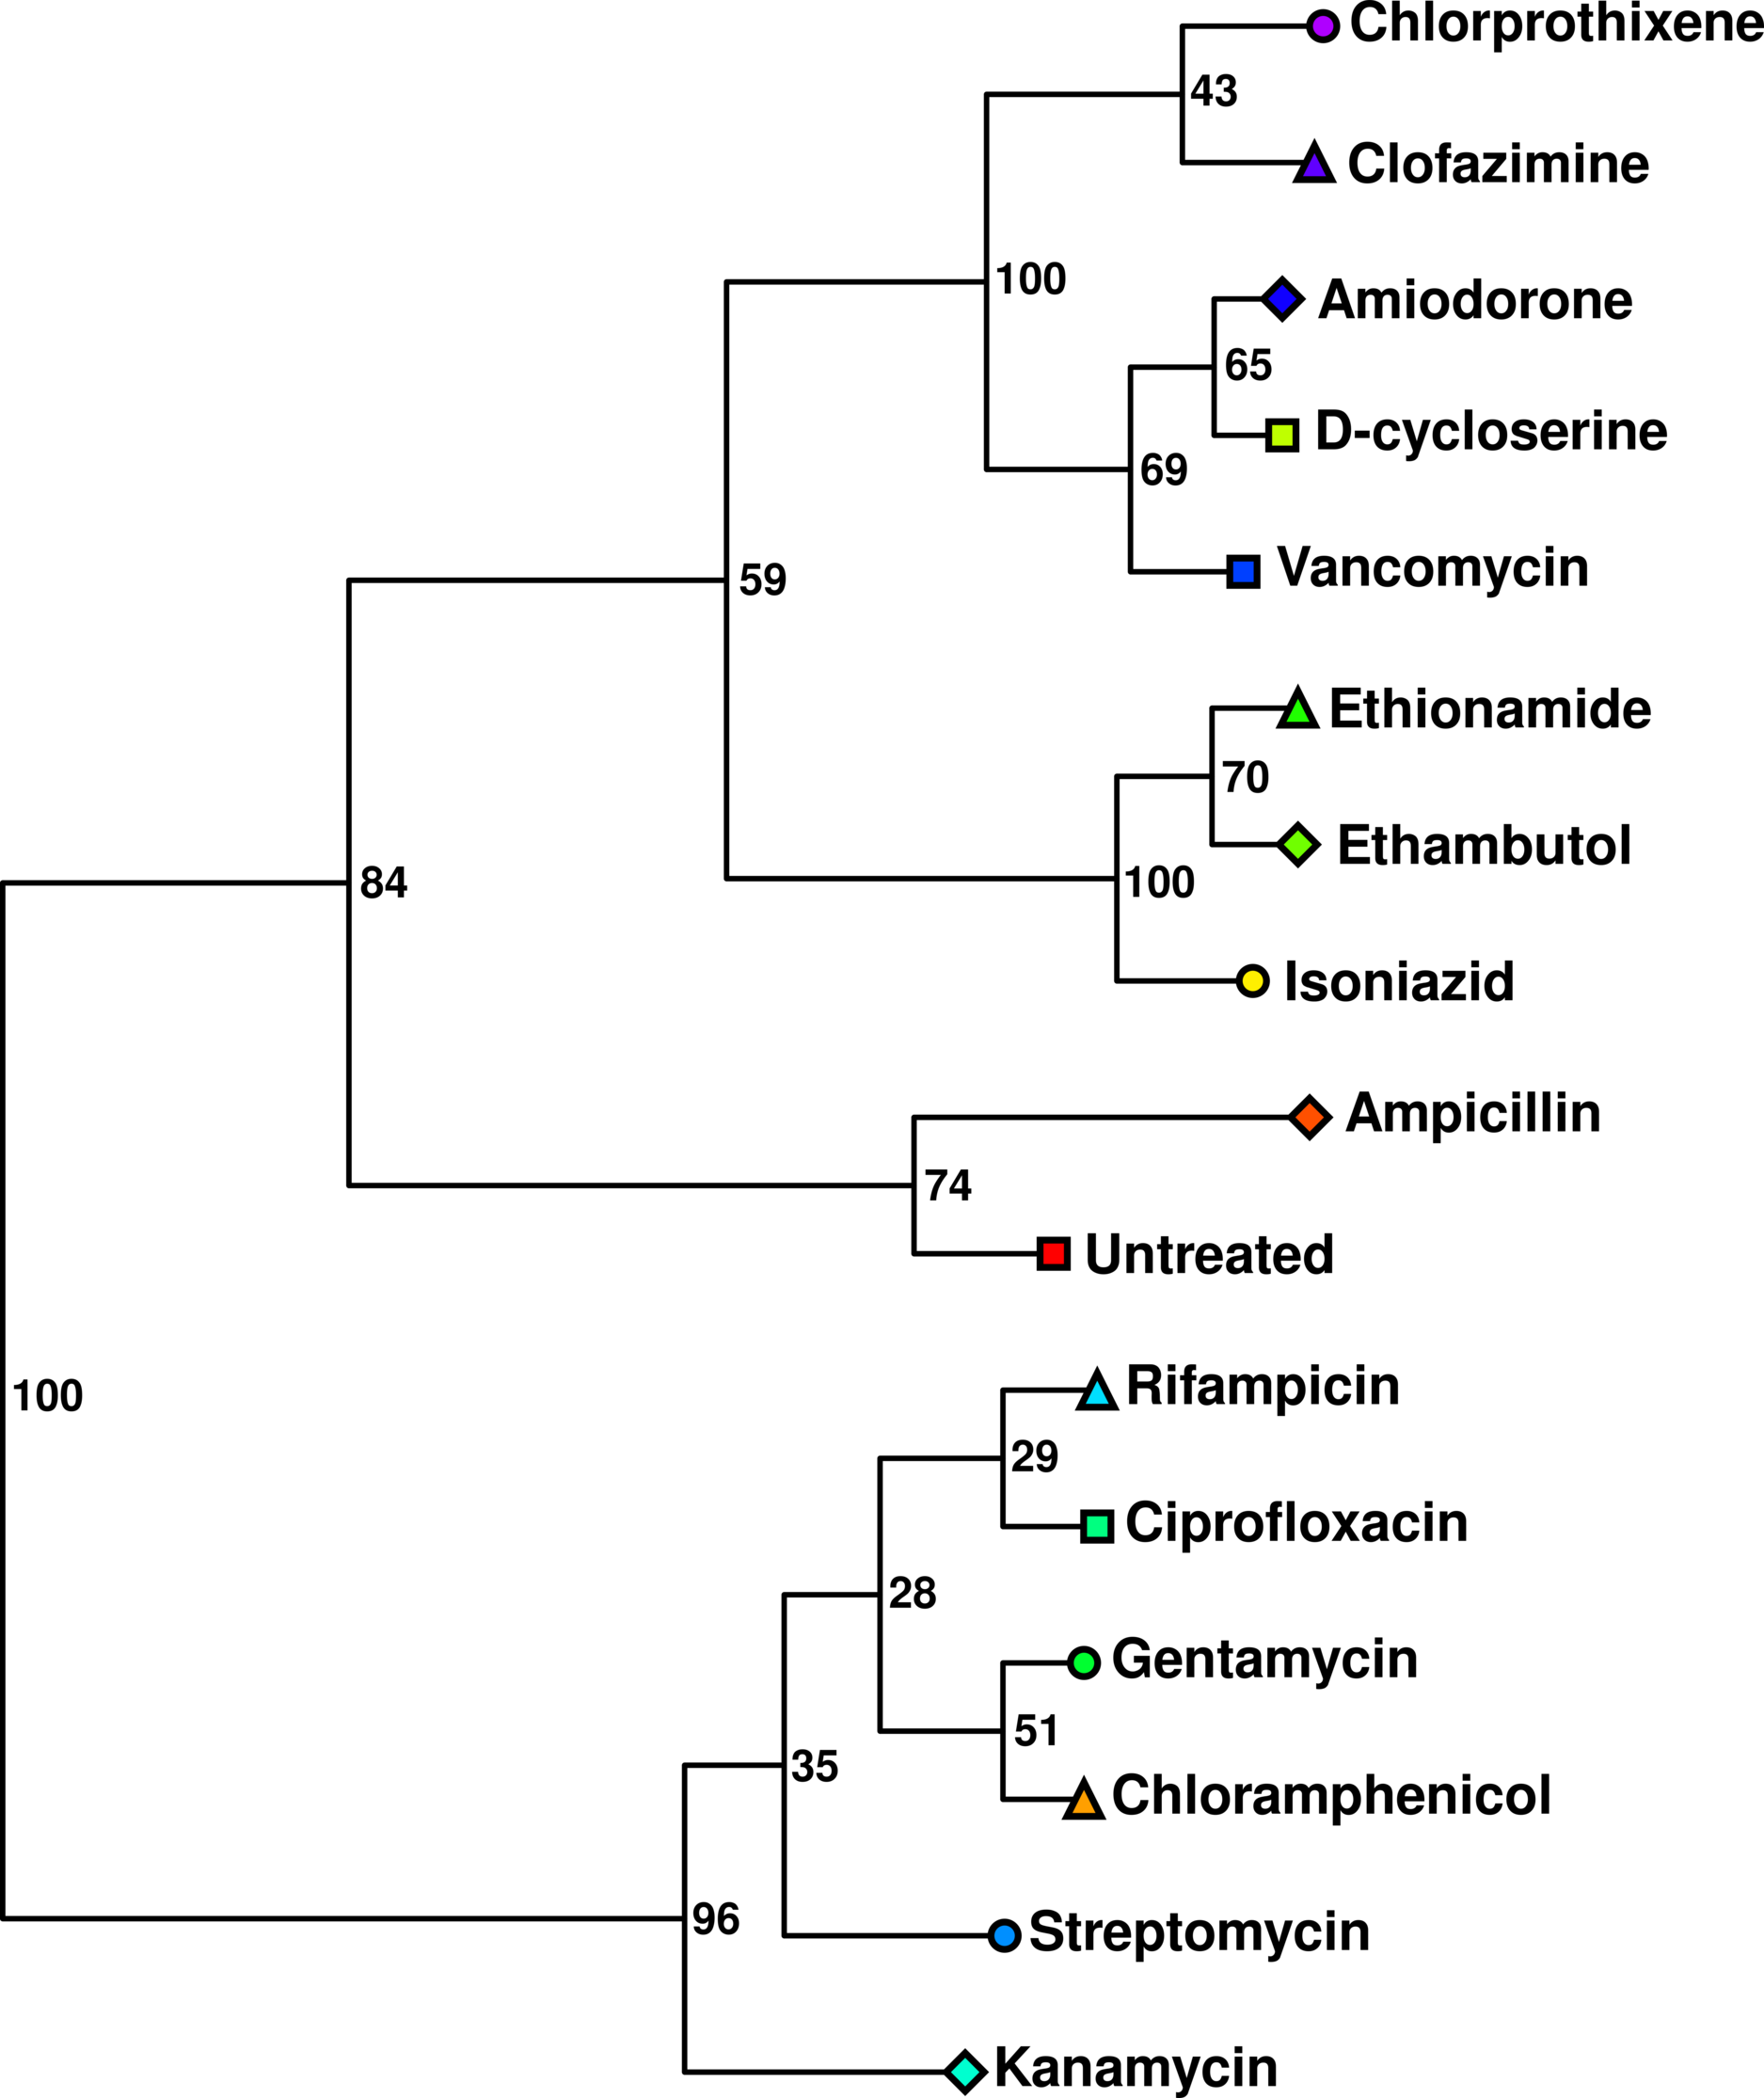
\includegraphics[width=3.5in]{figs/utils/03.png}
\caption
      [Dendrogram Generated using Euclidean Distances.]{
  {\bf Dendrogram Generated using Euclidean Distances.}
  \\
  Bootstrapped dendrogram generated from the scores data in Figure 8.1A using
  a Euclidean distance metric. Bootstrap statistics reported at each branch
  were computed from 5,000 bootstrap iterations.
}
\end{SCfigure}

\begin{doublespace}
It is important to note that our software is not a means of determining the
reliability of PCA or PLS-DA models, but only a toolset for quantifying the
scores that those models produce. In the case of PCA scores, significance of
the principal components used must be inferred based on the explained sum of
squares or another cross-validation technique
\cite{eastment:tech1982,krzanowski:biom1987}. PLS-DA models require
rigorous cross-validation to ensure model reliability, as they almost always
yield perfect separations between the scores of different groups
\cite{kjeldahl:jchemo2010}. With that in mind, separations between
groups not under discrimination may be due to true experimental differences in
PLS-DA scores plots, as opposed to the forced separations between discriminated
groups. Thus, the interpretation of any results from the PCA utilities must be
done with the knowledge of the underlying algorithm's mathematical intent, and
only after the model has been validated. While we demonstrated confidence
region generation using only 2D and 3D scores plots, it is important to note
that the PCA utilities software package places no restriction on the number of
components or on which components may be used during dendrogram generation and
$p$ value calculation. Any dimensionality or choice of scores may be used with
the described methods, provided all components are suitably validated.
\\\\
The updated and enhanced version of PCAtoTree, called PCA utilities, provides
a novel means of quantifying and visualizing separation significance in PCA,
PLS-DA and OPLS-DA scores plots. Importantly, PCA utilities enables single-step
methodologies for generating informative scores plots and dendrograms of
experimental groups in {\it any} study utilizing PCA, PLS-DA or OPLS-DA to
elucidate group structure in complex datasets, including metabolic
fingerprinting and nontargeted metabolic profiling. The tools are distributed
under version 3.0 of the GNU General Public License \cite{gpl3} and are freely
available at \url{http://bionmr.unl.edu/pca-utils.php}.
\end{doublespace}

\bibliographystyle{abbrv}
\bibliography{bworley}

